\section{Evaluation}

\subsection{Fixed-Wing Aircraft Example}

\begin{figure}[htb]	
    \begin{center}
    \centerline{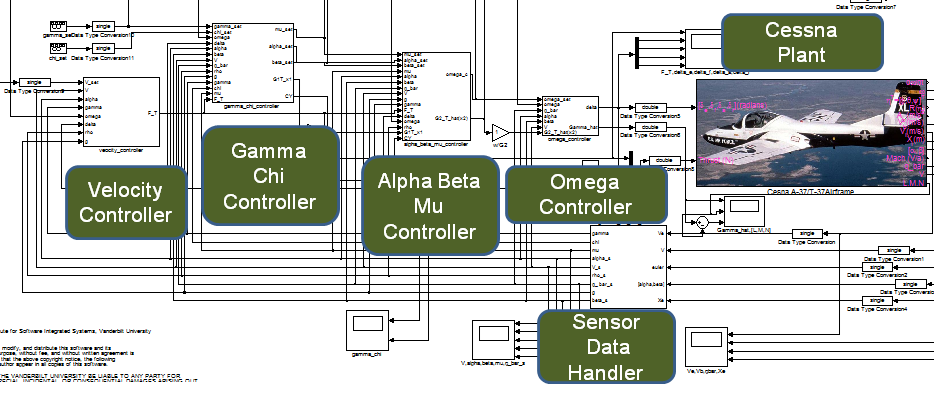
\includegraphics[width=\columnwidth]{figures/fixed_wing_controller_mdl.png}}
    \caption{Simulink Fixed Wing Controller Model}
    \label{fig:fw_simulink}
    \end{center}	
\end{figure}

\begin{figure}[htb]	
    \begin{center}
    \centerline{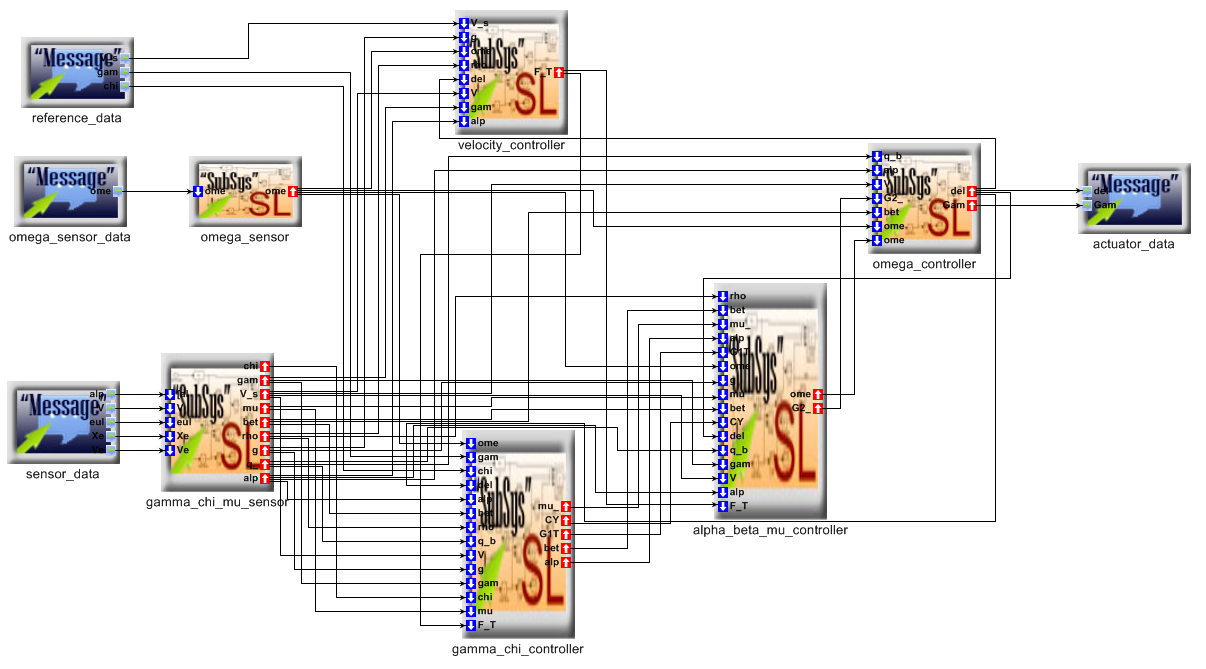
\includegraphics[width=\columnwidth]{figures/all_in_one}}
    \caption{Synchronous data flow for Fixed Wing Controller}
    \label{fig:sdfcontroller}
    \end{center}	
\end{figure}

Our case study covers cycle analysis of the control design for a fixed-wing 
aircraft.  The Simulink model (Fig. \ref{fig:fw_simulink}) shows the four controller blocks and the sensor data handler.  The particulars of the control architecture are not important for this example, but Kottenstette covers them in detail\cite{control:fixed_wing}.   The controller has five software functions which are specified as Simulink model blocks, and a dynamics component (the Cessna plant block).  The 
\textbf{MDL2MGA} model importer creates a structural replica of the Simulink
model in the ESMoL modeling language.  We use subsystems from the replica
to specify the function of synchronous software components.  
Fig. \ref{fig:sdfcontroller} illustrates one possible configuration of the fixed wing controller components.  
In this particular configuration 
(Fig. \ref{fig:sdfcontroller}) the entire dataflow is included in one
type definition, which means that the entire system will execute together
as a single synchronous function with all blocks firing at the same rate.
This particular configuration is useful for illustration, but is not the most practical implementation choice.  

% TODO: Describe the layers when we can get it working.
%In an ESMoL logical architecture model, specified software component types are
%instantiated to form a task-level dataflow model.  
%Simulink dataflow specifications.
%Component type definitions.
%Logical architecture - instances of component types (only warnings).
%Deployment models - actual malformed model detection for local dependencies.

\subsection{Incremental Analysis Results}

Table \ref{tab:cycletimes} contains data from the analysis of
the fixed wing model.  The first pass was performed incrementally, with each
subcomponent of the top level model analyzed first.  Then the top level is
analyzed using the stored path edges in the lower models.  The table reports
two run times for the analysis of each component -- the first is the processing time required to find the abstract cycles only, and the second is the full analysis which finds the expanded cycle for each abstract cycle (enumerating possibly multiple cycles per abstract cycle). The table also displays the number of hierarchical components visited and the number of individual model elements visited, together with the number of abstract cycles found and the total number of cycles.  The table row labeled \emph{top level (incremental)} contains the results for the analysis of the top level of the model once the individual path interfaces had been created for each of its subcomponents.  
The second pass (labeled \emph{top level (full)}) analyzed the entire fixed wing model at once, reporting the same quantities.  Our assessment of the scalability of the approach is inconclusive for three reasons -- 1) the model size is moderate, so overhead is likely large enough to be a significant factor in all of the run times, 2) we would need a comparison with time taken to process a fully flattened model, including the flattening traversals, and 3) we need to find larger models for our test set.  The analyzer found 18 abstract cycles and 54 detailed cycles at the top level for both passes.  The \emph{velocity\_controller} component also contained a single abstract cycle (consisting of two detailed cycles). Note that we analyzed for all cycles rather than only delay-free cycles to assess scalability. Total runtime was roughly equivalent between the full and
incremental methods for this particular model. The results so far are promising but inconclusive as far as improved performance.

\begin{table*}[htb]
\centering
\begin{tabular}[width=\columnwidth]{ | l | l | l | l | l | l | l | }

\hline
              & \textbf{Abstract} & \textbf{Full} &                     &                          & \textbf{Abstract} & \textbf{Total} \\
\textbf{Component} & \textbf{Run} & \textbf{Run}  & \textbf{Hier.} & \textbf{Total} & \textbf{Cycles} & \textbf{Cycles} \\
              & \textbf{Time (s)} & \textbf{Time (s)} & \textbf{Comps.}  & \textbf{Elts.} & \textbf{Found} & \textbf{Found} \\
\hline \hline
alpha\_beta\_mu\_controller & 0.9 & 0.9 & 9 & 80 & 0 & 0 \\
\hline
gamma\_chi\_controller & 1.6 & 1.6 & 7 & 134 & 0 & 0 \\
\hline
gamma\_chi\_mu\_sensor & 1.3 & 1.3 & 8 & 100 & 0 & 0 \\
\hline
omega\_controller & 0.9 & 0.9 & 9 & 80 & 0 & 0 \\
\hline
velocity\_controller & 0.6 & 0.8 & 6 & 60 & 1 & 2 \\
\hline
Top level (incremental) & 2.3 & 55.1 & 1 & 21 & 18 & 54 \\
\hline
Totals & 7.6 & 60.6 & & & 19 & 872 \\
\hline
 & & & & & & \\
\hline
Top level (full) & 7.9 & 60.5 & 42 & 554 & 19 & 56 \\
\hline
\end{tabular}
\caption{Cycle analysis comparisons for the fixed wing model.}
\label{tab:cycletimes}
\end{table*}

\begin{figure}[htb]	
    \begin{center}
    \centerline{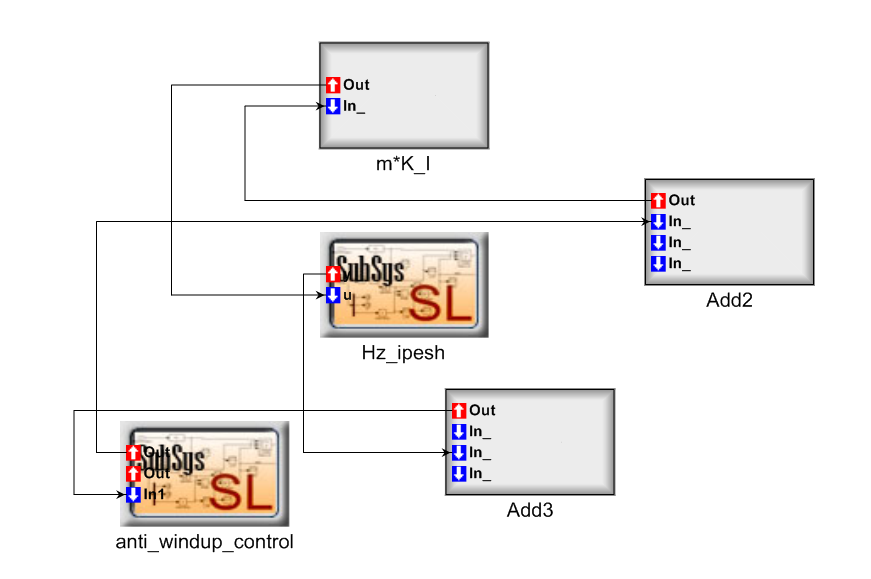
\includegraphics[width=\columnwidth]{figures/velocity_cycle.png}}
    \caption{Detail of the components involved in the cycle found in the velocity controller.}
    \label{fig:velcyclemod}
    \end{center}	
\end{figure}

\begin{figure}[htb]	
    \begin{center}
    \centerline{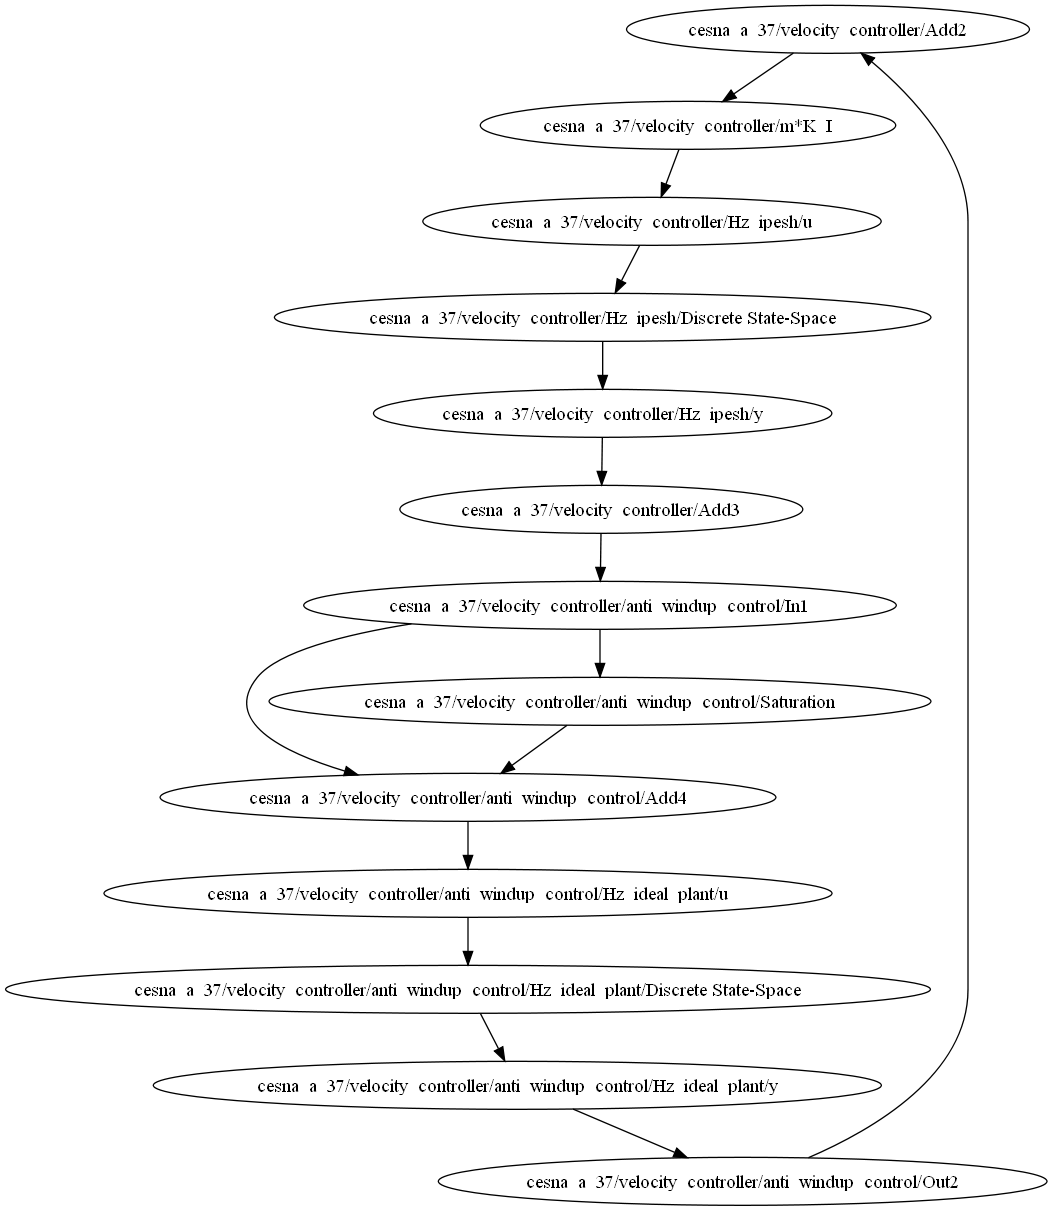
\includegraphics[width=\columnwidth]{figures/velocity_controller_cycle1.png}}
    \caption{Full cycle for the velocity controller.}
    \label{fig:velcycle}
    \end{center}	
\end{figure}

Figs. \ref{fig:velcyclemod} and \ref{fig:velcycle} display a subset of the \emph{velocity controller} component which contains a cycle, along with the expanded cycle for the component, in order to illustrate the cycle refinement in greater detail.
The abstract cycle search discovered the presence of a cycle within the component, but part of the cycle lies within a subcomponent (\emph{anti\_windup\_control}).  The cycle detection for \emph{anti\_windup\_control} created a single path
edge in the interface between the \emph{In1} port and the \emph{Out2} port, which corresponds to two paths within  \emph{anti\_windup\_control}.  The full 
cycle as shown (Fig. \ref{fig:velcycle}) is constructed in the analyzer, and then one more pass of Johnson's algorithm resolves the two cycles within the full cycle graph as reported in Tab. \ref{tab:cycletimes}.  The extracted cycle graph is much smaller (13 elements) than the corresponding fully flattened \emph{velocity controller} model, which would contain 60 elements.


